\section{Flag 00 - SQL Injection (Basic)}

\paragraph{10a16d834f9b1e4068b25c4c46fe0284e99e44dceaf08098fc83925ba6310ff5}
\begin{center}
    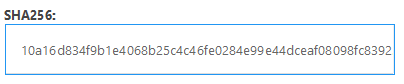
\includegraphics[width=0.5\textwidth]{03.Flag00/00-08.png}\\[0cm] 
\end{center}

The integrity of data and it's storage and retrieval is key to a successful
Web Application.

\subsection{Vulnerability}

The input bar allows a person to do raw database search with an open
'WHERE' clause for SQL Queries. This is dangerous as data remains unprotected. Countries
like South Africa have the POPI act which means that every effort must be made to keep
people's private information safe and free from a breach.

\subsection{Location}

http://<ip-address>:80/?page=member

\subsection{Method}

The way to get started is typing in an ID, it is an integer between
1 and $\infty$. You can see that ID for member 1 as shown in 
Figure~\vref{fig: 00-01 - Search start}. The next step is to try inject
your own SQL commands into the query\cite{W3Schools-SQLInjection}.

The next thing is to run '105 OR 1=1' as shown in Figure~\vref{fig: 00-02 - 105query}, the number 105 is arbitrary and can be
substituted with anything. You will see the results as shown in Figure~\vref{fig: 00-03 - 105query result}
which list everything in the database. You will notice that one of the Flags has first-name: "Flag"
Surname: "GetThe".

To see this illustrated properly just search user member '5'. This is shown in
Figure~\vref{fig: 00-04 - Get The Flag}. We have confirmation that the flag is
there.

The next step is finding the table names, run this command query
\begin{quote}
5 UNION SELECT TABLE\_NAME, COLUMN\_NAME FROM INFORMATION\_SCHEMA.COLUMNS
\end{quote}
and you will see the users, guestbook \& list\_images tables in the database. The
database that we are interested in, is the users table.

\begin{center}
    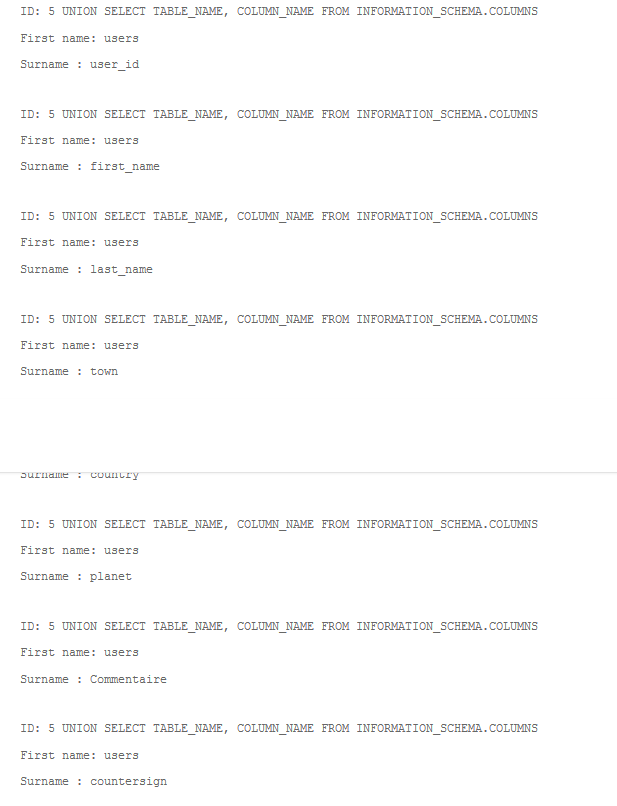
\includegraphics[width=0.5\textwidth]{03.Flag00/00-05.png}\\[0cm]    
\end{center}

You will have to run commands substituting the value of 'TABLE\_NAME' \&
COLUMN\_NAME  with the columns that you want. As shown in the
image of the query result. We are interested in only two columns in the
users table. 'Commentaire' and 'countersign' therefore we run this query
\begin{quote}
    5 UNION SELECT Commentaire, countersign FROM users
\end{quote}

\subsection{Tools}

\begin{figure}[!htb]
    \centering
    \subfloat[Search ID Member 1]{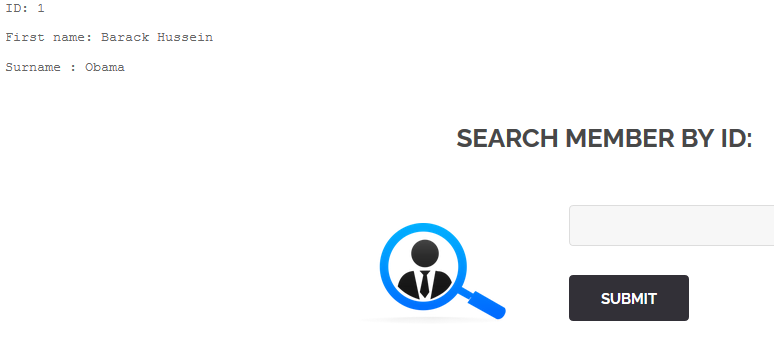
\includegraphics[width=.45\columnwidth]{03.Flag00/00-03.png}\label{fig: 00-01 - Search start}} \quad
    \subfloat[105 OR 1=1]{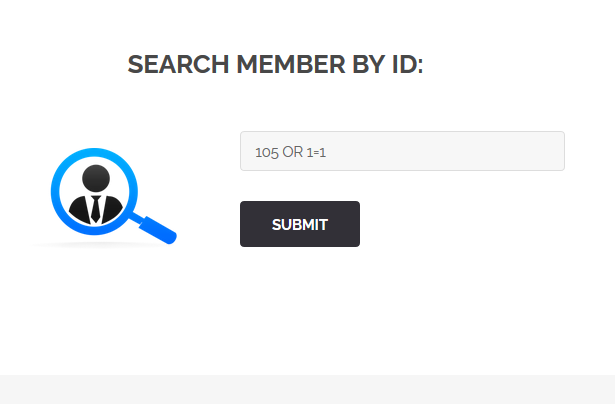
\includegraphics[width=.45\columnwidth]{03.Flag00/00-01.png}\label{fig: 00-02 - 105query}} \\
    \subfloat[Results of query]{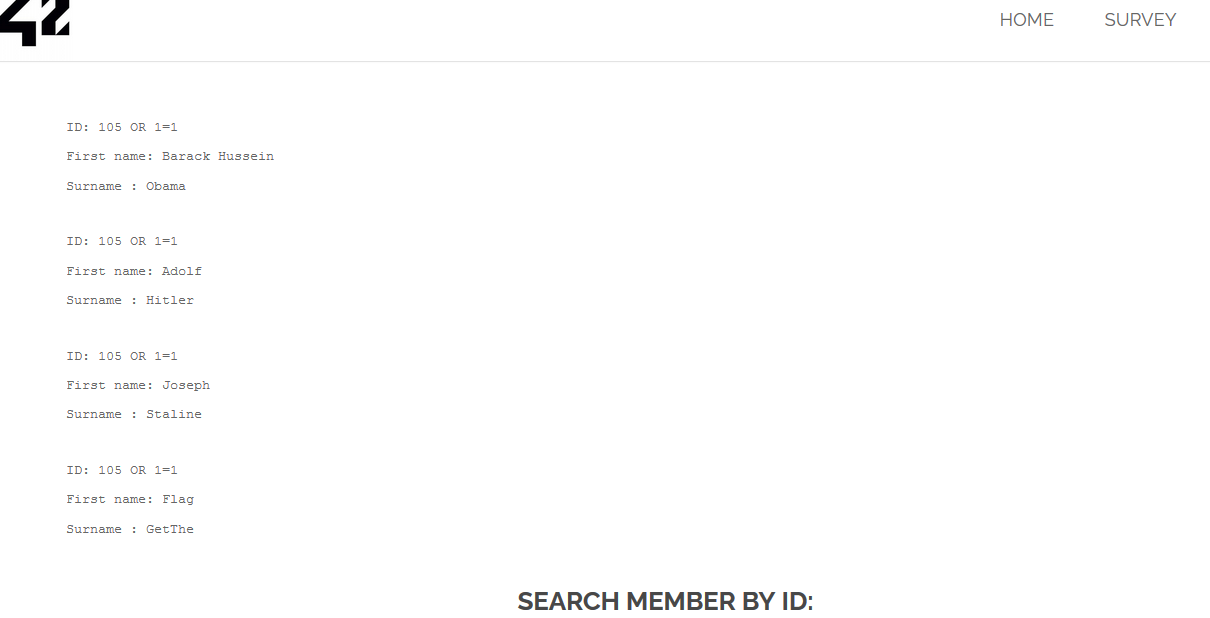
\includegraphics[width=.45\columnwidth]{03.Flag00/00-02.png}\label{fig: 00-03 - 105query result}} \quad
    \subfloat[Flag at Member Id: 5]{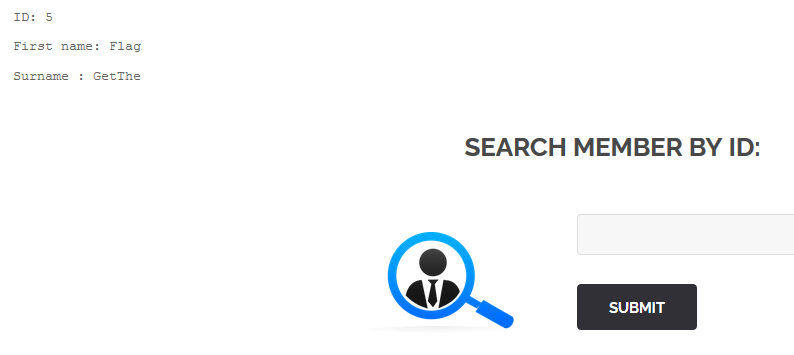
\includegraphics[width=.45\columnwidth]{03.Flag00/00-04.png}\label{fig: 00-04 - Get The Flag}}
    \subfloat[Secret Column Contents]{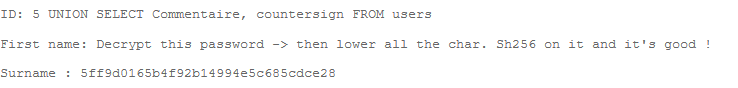
\includegraphics[width=.45\columnwidth]{03.Flag00/00-06.png}\label{fig: 00-06 - column content}} \quad
    \subfloat[MD5 Hash]{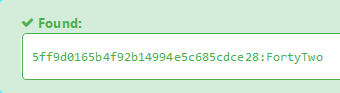
\includegraphics[width=.45\columnwidth]{03.Flag00/00-07.png}\label{fig: 00-07 - The Flag}}
    \caption[Flag 00 Method]{Process to Capture the SQL (Basic) Flag} % The text in the square bracket is the caption for the list of figures while the text in the curly brackets is the figure caption
    \label{fig:flag00 method}
\end{figure}
The tools used were \href{https://hashes.com/en}{hashes.com} and \href{https://www.owasp.org/index.php/SQL\_Injection}{OWASP} inlcuding
but not limited to the references cited in the Bibliography.

\subsection{Remedy}

\begin{itemize}
    \item Prepared Statements
    \item Sanitise
\end{itemize}